\documentclass{article}
\usepackage{blindtext}
\usepackage{amsmath,mathtools}
\usepackage{xcolor}
\usepackage{graphics,graphicx}
\usepackage{url}
\usepackage{amsmath}
\usepackage{mathtools}
\usepackage{array}
\usepackage{multicol}
\usepackage{multirow}
\usepackage{algorithmicx,algorithmic}
\usepackage{algpseudocode}
\usepackage{balance}
\usepackage{booktabs, makecell}
%All our required packages are included
\title{Karthik's \LaTeX Assignment}
\author{Karthik Kancharla \\
Computer Science and Engineering, IIT Dharwad\\

\texttt{190020020@iitdh.ac.in}}

\date{September 3, 2020}
\begin{document}
\tableofcontents
\listoffigures
\listoftables

\maketitle
\section{Our First Section}
%This is a section where i used blindtext which has no meaning related to the section.
This section will completely consist text.\\
\\
Here you will find some random information in the first section.
\\
\\
\blindtext
\\
\\
\texttt{\huge \textcolor{red}{My }College URL:}  \url{ www.iitdh.ac.in}
\\
\colorbox{yellow}{\textcolor{red}{\huge Our First Section Completed}}
\section{Our \textit{(Actually mine) }Mathematical Section}
This is our mathematical section. It mostly consists of mathematics :)\\
\subsection{Our First Mathematical Subsection}
Our inline Mathematical Expression: $E = mc^2$
\\
\\
Our Non-Numbered equation in a dedicated line: 

\begin{equation}
	(a+b)^2 = a^2 + 2ab + b^2\nonumber
	\label{eq: a+b}
\end{equation}
Our Non-Numbered equation in a dedicated line in a second way: 
\begin{align}
	(a+b)^2 = a^2 + 2ab + b^2 \nonumber
\end{align}
Our First Numbered equation in a dedicated line :
\begin{equation}
	(a-b)^2 = a^2 - 2ab +b^2 
	\label{eq: a-b}
\end{equation}
Our Multiline Equation: Area of Circle
\begin{align}
	 A & = {\pi r^2 }\\ \nonumber
	   & = \frac{\pi d^2 }{4}
\end{align}
\textcolor{blue}{Matrices:}\\
Matrix addition of A and B gives C.\\
where
A = 
$\begin{pmatrix}
	1 & 2 & 3\\
	4 & 5 & 6
\end{pmatrix}$
B = $\begin{pmatrix}
	1 & 1 & 1\\
	0 & 0 & 0
\end{pmatrix}$
and C = $\begin{pmatrix}
	2 & 3 & 4\\
	4 & 5 & 6
\end{pmatrix}$\\
\\
\textcolor{blue}{Square Root:}\\
Do you know $\sqrt{4}$ is equal to 2.\\
Do you know $\sqrt{mc^2}$ is equal to $\sqrt{m}$c.
\\
\textcolor{blue}{Summation:}\\
$\sum_{x=1}^{n}$ = $n(n+1)/2$
\\
\textcolor{blue}{Integration:}\\
$\int_{2}^{4}x = 6 + c$\\
\\
\textcolor{blue}{Nested Brackets with varying size:}\\
\\
$(\frac{1}{2})$ can also vary it's bracket size to $\big(\frac{1}{2}\big)$\\
An example of multiple brackets is:$( a - b\cos (\frac {c}{d}) )$
\\
\\

\textcolor{blue}{Fractions:}
\\
Do you know that the fraction $\frac{2}{4}$ is equal to $\frac{1}{2}$ and the value of it is 0.5. Here fraction is converted to the decimal value from numerator and denominator.

%And then in this way our mathematical section completes. Time for Celebration.
\section{Tables}
%This is our tables section.
\textcolor{red}{\huge \textit{This is not a Dining Table!}}
\begin{table}

\begin{center}
	\begin{tabular}{ccc}
		\hline
		\multirow{2}{*}{Our Sir in Google Meet}&Student A\\
		&Student B\\
		\hline
		\label{tab: gmeet}
		Student C&Student D&Student KARTHIK\\
		\hline
	\end{tabular}
\end{center}

\caption{Google Meet Interface as a Table with Teacher}
\end{table}
\\
\\
The table number ~\ref{tab: gmeet} shows teacher interacting with students in Google Meet interface.\\
\\

\begin{table}
	
	\begin{center}
		\begin{tabular}{cc}
			\hline
			\multicolumn{2}{c}{Students}\\
			A&B\\
			\hline
			\label{tab: gmeetstud}
		\end{tabular}
	\end{center}
	
	\caption{Google Meet Interface without Teacher}
\end{table}
The table number ~\ref{tab: gmeetstud} shows students in Google Meet interface.\\
\\ 
One Sample table:
\begin{table}[h]
	\begin{center}
		\caption{My Sample Table}
		\label{tab: mysampletable}
		\begin{tabular}{l|S|r|l}
			\textbf{Value 1} & \textbf{Value 2} & \textbf{Value 3} & \textbf{Value 4}\\ 
			\hline
			1 & 5 & 6 & 8\\ 
			2 & 9 & 11 & 13\\ 
			3 & 58 & c & 62\\ 
		\end{tabular}
	\end{center}
\end{table}
\section{Information from Images}

\textbf{In Figure~\ref{fig:aryabhatta}, We see one of the World's Greatest Mathematicians \textcolor{red}{Aryabhatta}.}\\

Aryabhata is the author of several treatises on mathematics and astronomy, some of which are lost.

His major work, Aryabhatiya, a compendium of mathematics and astronomy, was extensively referred to in the Indian mathematical literature and has survived to modern times. The mathematical part of the Aryabhatiya covers arithmetic, algebra, plane trigonometry, and spherical trigonometry. It also contains continued fractions, quadratic equations, sums-of-power series, and a table of sines.

The Arya-siddhanta, a lost work on astronomical computations, is known through the writings of Aryabhata's contemporary, Varahamihira, and later mathematicians and commentators, including Brahmagupta and Bhaskara I. This work appears to be based on the older Surya Siddhanta and uses the midnight-day reckoning, as opposed to sunrise in Aryabhatiya. It also contained a description of several astronomical instruments: the gnomon (shanku-yantra), a shadow instrument (chhAyA-yantra), possibly angle-measuring devices, semicircular and circular (dhanur-yantra / chakra-yantra), a cylindrical stick yasti-yantra, an umbrella-shaped device called the chhatra-yantra, and water clocks of at least two types, bow-shaped and cylindrical.\\
\begin{figure}
	\begin{center}
		
		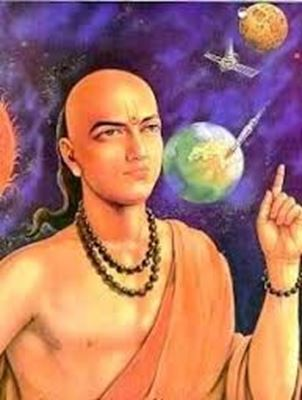
\includegraphics[width=0.50\textwidth]{aryabhatta}
		\caption{Aryabhatta}
		\label{fig:aryabhatta}
		
	\end{center}
\end{figure}
\begin{figure}
	\begin{center}
		
		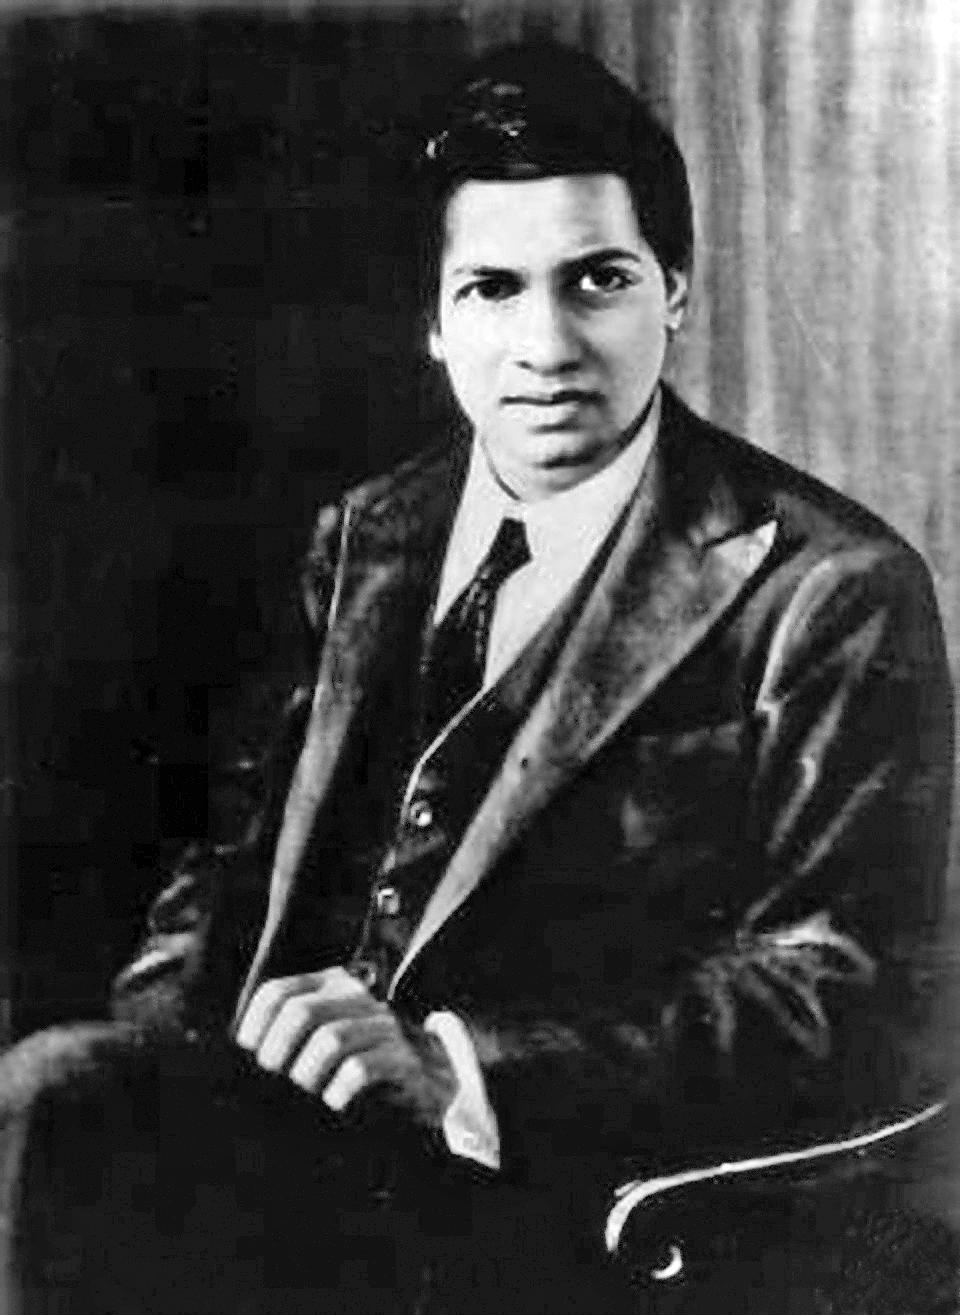
\includegraphics[width=0.50\textwidth]{Srinivasa}
		\caption{Srinivasa Ramanujan}
		\label{fig:ramanujan}
		
	\end{center}
\end{figure}
\\
\textbf{In Figure~\ref{fig:ramanujan}, We see one of the finest Indian Mathematicians \textcolor{red}{Srinivasa Ramanujan}.}\\

Though he had almost no formal training in pure mathematics, he made substantial contributions to mathematical analysis, number theory, infinite series, and continued fractions, including solutions to mathematical problems then considered unsolvable. Ramanujan initially developed his own mathematical research in isolation: according to Hans Eysenck: "He tried to interest the leading professional mathematicians in his work, but failed for the most part. What he had to show them was too novel, too unfamiliar, and additionally presented in unusual ways; they could not be bothered".[4] Seeking mathematicians who could better understand his work, in 1913 he began a postal partnership with the English mathematician G. H. Hardy at the University of Cambridge, England. Recognizing Ramanujan's work as extraordinary, Hardy arranged for him to travel to Cambridge. In his notes, Hardy commented that Ramanujan had produced groundbreaking new theorems, including some that "defeated me completely; I had never seen anything in the least like them before", and some recently proven but highly advanced results.




\section {Lists of Random Things}
\subsection{Mathematicians}
\label{sec: mathemat}
You can see their info mentioned in the section \ref{sec: mathemat}
\begin{itemize}
	\item Aryabhatta
	\item Srinivasa Ramanujan
	\item Euler
	\item Euclid
	\item Pythagorean
	\item \texttt{\textcolor{red}{\huge Karthik Kancharla, Yes it's me:)}}
	
\end{itemize}
\subsection{Top Telugu Movies}
\begin{enumerate}
	\item Baahubali 1
	\item Baahubali 2
	\item Sarileru Neekevvaru
\end{enumerate}
\subsection{Super Heroes with cross referencing}
\label{subsec: super}
\begin{description}
	\item[Iron Man] Wears an iron man suit. Iron man suit works due to following formula mentioned in equation number \ref{eq: a+b} calculated by famous mathematician in figure \ref{fig:aryabhatta}
	\item[Thor] Doesn't wear an iron man suit, because he doesn't like it due to the formula mentioned in equation number \ref{eq: a-b} calculated by famous mathematician in figure \ref{fig:ramanujan}
\end{description}
\section{Info about References}
This reference number \cite{Bruchezeabb3753} is a good article, it is the first article I found on web. It's very interesting.
\\
%Section containing references.
This reference number \cite{10.1093/ibd/izaa212} is the second article about science.
\\
Also the article in reference \cite{10.1093/ndt/gfaa170} is also a good article on science to read in this pandemic, try it for sure.
\\
The articles in the references \cite{Collins603} and \cite{Thorp885} correspond to the latest infomation about covid vaccines and cures correspondingly.
\section{Quick Sort Algorithm}
This doesn't come into sub section \ref{subsec: super} and here we don't discuss about super heroes. Pseudo code of Quick Sort Algorithm goes as follows:
\\
\\
\\
It contains 2 functions: Pseudo Codes of both the functions are as follows.
\\
low is starting index, high is ending index, pi is partition index.\\
\\
This function takes last element as pivot, places
the pivot element at its correct position in sorted
array, and places all smaller (smaller than pivot)
to left of pivot and all greater elements to right
of pivot.\\
\begin{algorithmic}
	%low is starting index, high is ending index, pi is partition index
	\Function{quicksort}{$arr[],low,high$}
	\If{$low \leq high-1 $}
	\State $pi \gets \Call{partition}{arr,low,high}$
	\State \Call{quicksort}{$arr[],low,pi-1$}
	\State \Call{quicksort}{$arr[],pi+1,high$}
	\EndIf
	\Return
	\EndFunction
	\\
	%This function takes last element as pivot, places
	%the pivot element at its correct position in sorted
	%array, and places all smaller (smaller than pivot)
	%to left of pivot and all greater elements to right
	%of pivot
	\Function{partition}{$arr[],low,high$}
	\State $pivot$ $\gets$ $arr[high]$
	\State $i \gets (low-1)$
	\For{$j \gets low; j\leq (high-1);\ j \gets j+1$}
	\If{$arr[j] \leq pivot-1$}
	\State $i \gets i+1$
	\State \Call{swap}{$arr[i], arr[j]$} 
	\EndIf
	\EndFor
	\EndFor
	\Call{swap}{$arr[i+1], arr[high]$}
	\State \Return $(i+1)$
	\EndFunction
	
	
\end{algorithmic}

\pagecolor{green}
\bibliography{bibtekref.bib}
\bibliographystyle{ieeetr}
\colorbox{yellow}{\textcolor{red}{\huge All Sections Completed and All Tasks Done.}}
First some pages are specifically set to white because I don't like coloured pages in my Document.
%The End




\end{document}
